\section{问题二：异构无人机多点多架次运输调度}
\subsection{问题分析}
\subsubsection{由独立组批到耦合调度}
问题二取消“单服务区直接往返”的限制，允许一次飞行串访多个服务区，并要求明确实体无人机、电池和开始时刻。与问题一相比，新增自由度能够减少重复返航，却也引入三类耦合：访问顺序改变每箱交付时刻；前站卸货改变后续航段的剩余载荷和能耗；实体机与共享电池的再次可用时刻又决定任务能否并行。因而，问题二不是把问题一的18个批次简单排队，也不是普通的容量车辆路径问题。

题目中的医疗与首批保障要求具有硬约束性质，而一般物资的期望时间用于评价服务质量。若把两类时限放入同一个加权罚函数，算法可能用多个紧急箱迟到换取较短总路程，这与应急保障逻辑不符。因此本文先把硬违约数固定为0，再在可行集合内评价一般物资迟到、完工时间、能耗和架次数。

\subsubsection{关键决策与难点}
问题二需要同时确定六类决策：货箱属于哪个架次、同一架次访问哪些服务区、访问顺序如何、采用何种机型、分配哪架实体机与哪块同型电池、何时开始准备。前四类决定任务本身的持续时间和能耗，后两类决定任务能否在资源时间轴上落地。若只先求路线再任意分配资源，可能出现硬时限可行的抽象路线因电池尚未充满而无法按时起飞。

另一个难点是“到达”与“交付完成”不同。无人机抵达服务区后需要基础作业和逐箱交接，同站不同货箱的完成时刻并不相同；以到达时刻判断截止会系统性低估后排货箱的延误。本文保留站内交接顺序，并在每次卸货后更新剩余载荷，使时间和能量沿同一访问序列同步递推。

\subsubsection{求解框架选择}
完整问题同时含集合划分、异构车辆路径、时间窗和双资源排程，直接建立大规模混合整数模型会产生大量“货箱—架次—顺序—实体—电池—时刻”组合变量。考虑到题目规模和硬时限可行性的重要性，本文采用分层构造方法：分别建立硬箱专送基线与同目的地混装方案，对剩余软箱执行单区精确组批和异区双点串访合并，最后用事件仿真器分配实体机和满电电池。两套方案均重新计算完整物理量，不以距离近似替代能量和时限复核。

\subsection{时限—能量—资源统一模型}
\paragraph{决策表示与硬软时限}
将运输架次$r$表示为机型$g_r$、访问序列$\pi_r$、货箱集合$B_r$、实体机$u_r$、共享电池$k_r$及准备开始时刻$s_r$。每个货箱必须恰属于一个架次，并在自身目的服务区交付；机型与实体机、电池类型必须匹配。

对医疗箱和首批保障箱定义适用截止集合$\mathcal D_b$：医疗箱加入期望时刻，首批箱加入首批截止。硬时限箱满足
\begin{equation}d_b^{hard}=\min\mathcal D_b,\qquad C_b\le d_b^{hard}.\end{equation}
对$\mathcal D_b=\varnothing$的软时限箱，仅在目标中评价归一化加权迟到：
\begin{equation}
WTD=\sum_{b\in B^{soft}}\alpha_b\frac{\max(0,C_b-d_b^{exp})}{d_b^{exp}}.\label{eq:wtd}
\end{equation}
这里的“送达”采用完成该箱交接的时刻$C_b$，并非无人机到达服务区的时刻。这样的区分在同站多箱交接时会影响临界货箱是否逾期。

\paragraph{逐站时刻与剩余载荷递推}
令$\pi_r=(i_1,\ldots,i_m)$，$i_0=O01$，起飞时刻为
\begin{equation}\tau_{r0}^{dep}=s_r+t_{g_r}^{prep}+|B_r|t_{g_r}^{load}.\end{equation}
到达第$j$个服务区、完成站内投送和离开的时刻依次为
\begin{align}
\tau_{rj}^{arr}&=\tau_{r,j-1}^{dep}+t_{g_r,i_{j-1},i_j},\\
C_b&=\tau_{rj}^{arr}+t_{g_r}^{base}+\ell_b t_{g_r}^{handover},\\
\tau_{rj}^{dep}&=\tau_{rj}^{arr}+t_{g_r}^{base}+|B_{ri_j}|t_{g_r}^{handover}.
\end{align}
其中$\ell_b$为货箱在该站的交接序号。按有效硬截止升序、应急优先系数降序、编号升序排列，软时限箱在硬时限箱后依上述规则交接。离站后扣除本次交付质量，再用新的剩余载荷计算下一航段能耗。末站离开后加返航时间，得到$\tau_r^{ret}$。

这一递推把访问顺序同时作用于时间和能耗：较早卸下重箱可减轻后续载荷，但可能推迟其他节点的硬时限箱。多点路线必须逐段重算，不能仅在两个单点能耗之间做距离修正。

\paragraph{实体机与电池的双资源约束}
运输实体机在半开区间$[s_r,\tau_r^{ret})$被占用；电池还需完成返航后的充电，因此其占用区间为
\begin{equation}I_r^{bat}=[s_r,\tau_r^{ret}+T^{chg}(SOC_r^{end})).\end{equation}
对每个实体机$u$和电池$k$，同一时刻分别满足
\begin{equation}
\sum_{r:u_r=u}\ind_{[s_r,\tau_r^{ret})}(t)\le1,\qquad
\sum_{r:k_r=k}\ind_{I_r^{bat}}(t)\le1.
\end{equation}
半开区间使“上一任务结束的瞬间开始下一任务”不会被重复计为冲突。题面未另给运输机周转时长，实体机返回后可开始准备；其原电池仍在充电时，可以换用已经满电的同型电池。

图\ref{fig:q2-resource}用符号时刻说明两类资源的差异。机体可再次执行并不意味着原电池可再次使用；这也是仅按无人机架数排列甘特图不足以检验资源可行性的原因。
\begin{figure}[htbp]\centering
\begin{tikzpicture}[x=.8cm,y=1cm,font=\small]
\draw[edge](0,0)--(13,0) node[right]{时间};
\node[anchor=east] at(0,1.2){实体机};\node[anchor=east]at(0,2.3){电池};
\filldraw[fill=blue!12,draw=blue!50] (1,.8) rectangle (7,1.6);
\node at(4,1.2){准备、飞行、交付与返航};
\filldraw[fill=blue!12,draw=blue!50] (1,1.9) rectangle (7,2.7);
\filldraw[fill=orange!15,draw=orange!60] (7,1.9) rectangle (12,2.7);
\node at(4,2.3){执行任务};\node at(9.5,2.3){返航后充电};
\foreach \x in {1,7,12}{\draw[dashed,gray](\x,0)--(\x,2.8);}
\node[below]at(1,0){$s_r$};\node[below]at(7,0){$\tau_r^{ret}$};
\node[below]at(12,0){$\tau_r^{ret}+T^{chg}$};
\end{tikzpicture}
\caption{运输机与共享电池占用差异示意；横向长度不代表实际计算时长}\label{fig:q2-resource}
\end{figure}

\subsection{求解流程与指标权衡}
\paragraph{分层评价指标}
在全部硬约束成立的集合内，以$(WTD,C_{max},E_T,N_T)$作为分层比较指标，其中
\begin{equation}C_{max}=\max_r\tau_r^{ret},\quad E_T=\sum_rE_r,\quad N_T=|\mathcal R|.\end{equation}
先保证医疗与首批交付，再比较一般物资及时性；在及时性相同的候选中依次减少完工时间、能耗和架次数。该目标定义评价偏好，并不意味着构造算法已经穷尽其可行集合。

\paragraph{基线与混装方案构造}
求解先构造硬箱专送基线并确定紧迫批次的实体机指派，再据此形成同目的地混装方案：对各服务区枚举普通货箱补入组合，补入后的架次重新核验质量、体积、逐段递减载荷能耗、返航余量及每个硬时限，并保持硬时限箱优先交接。剩余货箱执行单服务区精确组批，随后把能够节能的两个异区单点任务贪心合并为双区串访。该构造吸收了带时间窗路径问题“先保证可行、再组合任务”的思想\textsuperscript{\cite{Ropke2006}}，但当前程序并未实现通用大邻域搜索。

两套方案均依次执行三项确定性操作：同目的地软箱补入、剩余软箱精确组批、异区单点任务节能合并；合并时比较两种访问顺序。随后分别完成实体资源排程，并按$(N_{late}^{hard},WTD,C_{max},E_T,N_T)$字典序比较整套结果。因程序只在这两套构造中择优，结论表述为“当前构造方案优于所列基线”，不宣称已搜索全部拆分与合并组合。

\paragraph{事件仿真与资源落地}
对每种机型分别维护实体机可用时刻$a_u$和电池满电时刻$a_k$。当一个抽象运输任务$r$进入排程时，枚举同型实体机—电池组合，其最早准备开始时刻为
\begin{equation}
s_r(u,k)=\max\{a_u,a_k,r_r^{release}\},
\end{equation}
其中$r_r^{release}$表示由硬截止逆推或波次约束给出的最早释放要求。将$s_r(u,k)$代入完整路线递推，得到逐箱交付、返航SOC与充电结束时刻；对容量和能量可行的组合，按硬迟到箱数、最大硬迟到、软时限代价、交付时刻、能耗和资源恢复时刻依次评分，然后更新$a_u$和$a_k$。这一过程把“选哪个任务”与“任务何时能够真实执行”分开处理；最终方案再统一核验硬迟到为0。

事件仿真的核心步骤为：
\begin{enumerate}
  \item 按硬截止、任务紧迫度和候选增量代价选择下一待排任务；
  \item 枚举同型实体机与电池，计算最早可开始时刻；
  \item 逐站递推到达、交付、离开、返航、SOC和充电完成；
  \item 容量或返航余量不可行的组合不进入评分；对其余组合计算硬迟到、软迟到及资源恢复指标；
  \item 接受评分最小的组合，写入任务、交付和资源事件表，并在最终方案核验硬迟到为0；
  \item 所有任务完成后执行覆盖守恒与区间冲突扫描。
\end{enumerate}

图~\ref{fig:q2-flow}给出问题二从货箱分层到资源事件审计的完整流程。容量或能量检查不通过的路线不进入资源评分；硬时限偏差则作为评分的最高优先级，并在整套方案形成后再次核验。
\begin{figure}[H]\centering
\begin{tikzpicture}[node distance=6mm]
\node[block,text width=7.4cm](input){读取货箱、机型、实体机、电池与DEM\\划分硬时限箱和软时限箱};
\node[block,text width=7.4cm,below=of input](seed){构造硬箱专送基线\\确定紧迫任务与实体机指派};
\node[block,text width=7.4cm,below=of seed](mix){枚举软箱补入、单区组批与双区串访\\逐站更新剩余载荷和交付时刻};
\node[block,text width=7.4cm,below=of mix](feas){检查质量、体积、DEM净空、返航SOC与硬时限};
\node[block,text width=7.4cm,below=of feas](event){事件仿真分配实体机与满电电池\\传播返航、充电和再次可用时刻};
\node[block,text width=7.4cm,below=of event](select){与硬箱专送基线按字典序比较\\输出路线、逐箱交付与资源时间轴};
\draw[edge](input)--(seed);\draw[edge](seed)--(mix);\draw[edge](mix)--(feas);
\draw[edge](feas)--node[right,font=\small]{通过}(event);\draw[edge](event)--(select);
\draw[edge](feas.east)--++(1.1,0) node[right,font=\small]{不通过} |- (mix.east);
\end{tikzpicture}
\caption{问题二异构运输调度求解流程}\label{fig:q2-flow}
\end{figure}

\subsection{调度结果与对比分析}
\paragraph{基线设置与总体指标}
基于修正后的DEM穿越像元高程口径，表~\ref{tab:q2-compare}给出两套构造方案的实算比较。两者均完成80箱唯一交付，31箱硬时限货箱均无违约；混装方案把普通物资超期箱数由23箱降至9箱，并同时减少架次、完成时间和能耗，故选作问题二当前方案。
\begin{table}[htbp]
  \centering
  \caption{问题二基线与硬软混装方案比较}
  \label{tab:q2-compare}
  \begin{tabular}{lrrrrrr}
    \toprule
    方案 & 硬违约/箱 & 普通超期/箱 & $WTD$ & $C_{max}$/h & $E_T$/kWh & 架次 \\
    \midrule
    硬箱专送基线 & 0 & 23 & 111.492 & 3.527 & 83.012 & 26 \\
    硬软混装方案 & 0 & 9 & 38.787 & 2.679 & 69.602 & 22 \\
    \bottomrule
  \end{tabular}
\end{table}

\paragraph{资源时间轴与可执行性}
图~\ref{fig:q2-gantt}进一步给出所选22架次在8架实体运输机和14块共享电池上的实际占用区间。上图浅色段为起飞前准备与装载，深色段为起飞至返航；下图彩色段为电池执行任务，灰色段为返航后的两阶段充电。任一实体机的任务区间均不重叠，同一电池的新任务也均在上一充电区间结束后开始。全部运输机于2.679~h前返航，最后一块电池于3.386~h完成充电，因此运输完工时间与资源完全恢复时间应分别报告。

\begin{figure}[H]
  \centering
  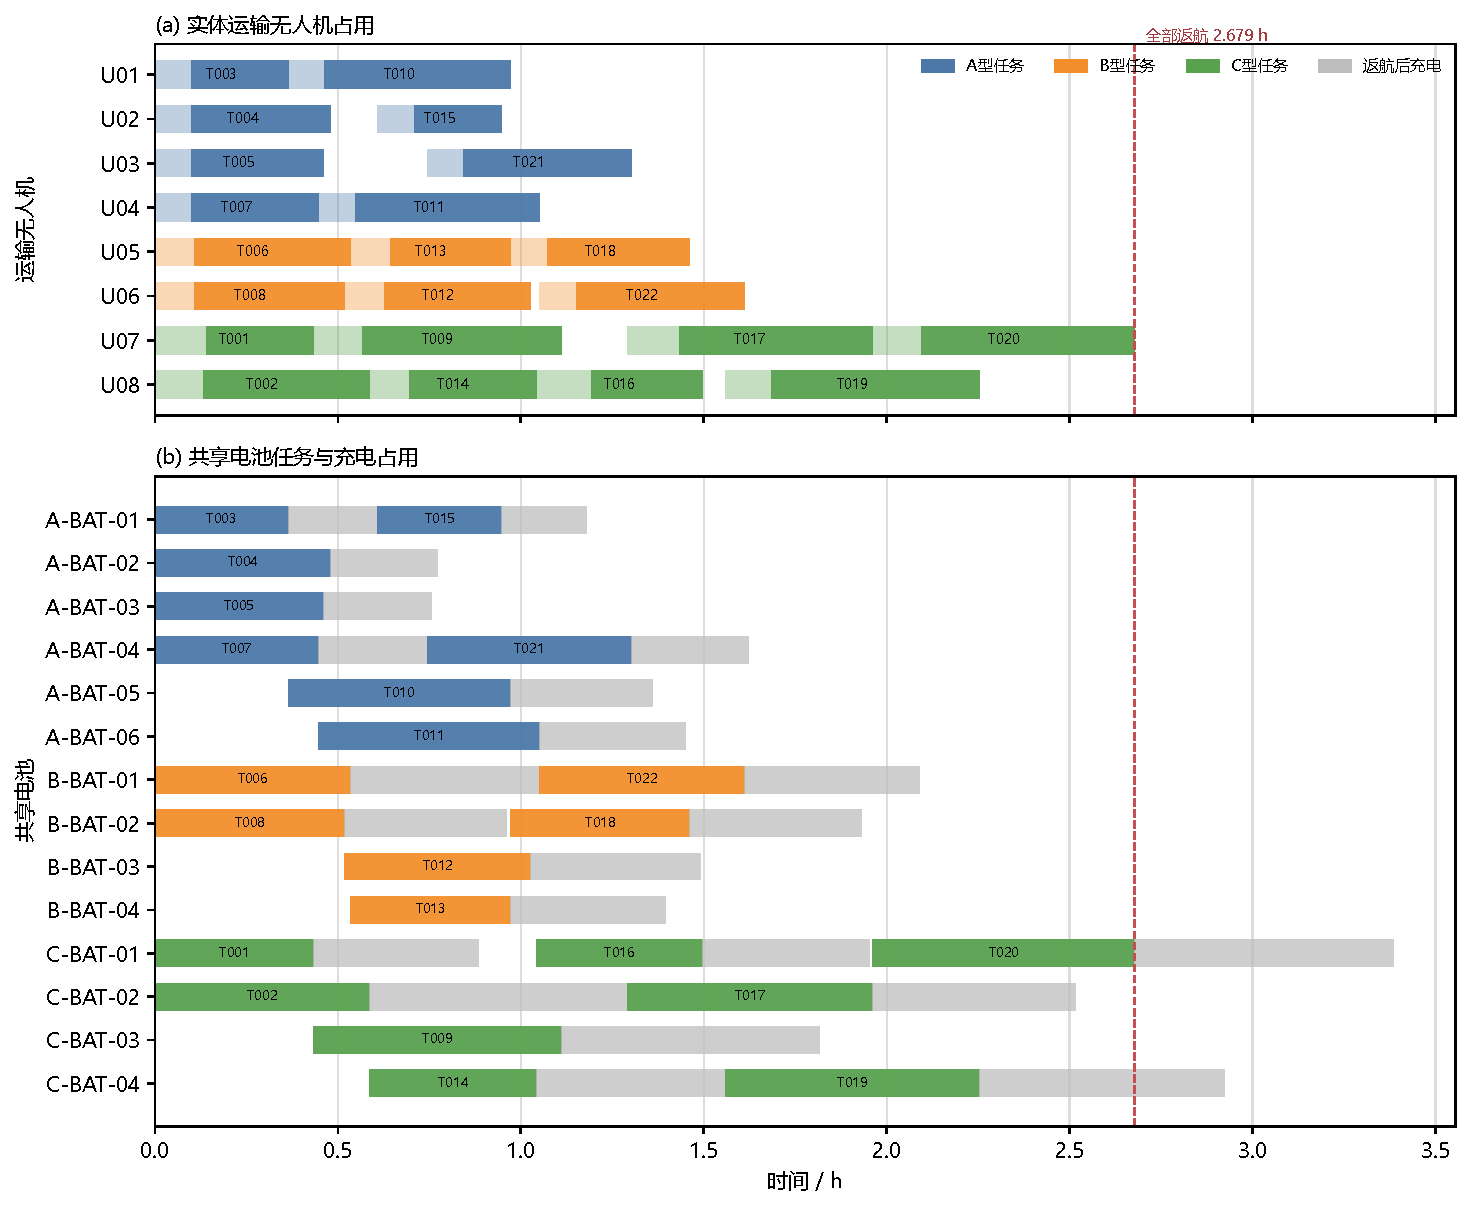
\includegraphics[width=\textwidth]{figures/q2/q2_resource_gantt.pdf}
  \caption{问题二运输无人机与共享电池联合甘特图。浅色段表示起飞前准备与装载，彩色段表示任务占用，灰色段表示返航后充电，红色虚线为全部运输架次返航完成时刻。}
  \label{fig:q2-gantt}
\end{figure}

\paragraph{改进幅度及其原因}
相对基线，混装方案的$WTD$下降65.2\%，全部返航完成时间缩短24.1\%，总运输能耗下降16.2\%，架次下降15.4\%。

四项指标同步改善的主要原因不是提高飞行速度，而是减少重复的准备、装载、爬升、返航和基础交接过程。把目的地相同的软箱补入已有紧急任务，可利用原本闲置的质量与体积；少量双区串访则在硬时限允许时减少一次完整往返。与此同时，方案仍有9个一般物资箱超过期望时刻，说明硬截止优先会把有限的早期机体与满电电池配置给紧急箱。该权衡是目标层次的直接结果，而不是程序漏排。

需要强调的是，22架次大于问题一的18架次并不矛盾。问题一允许各服务区独立比较组批，累计时间也不受实体资源和时限约束；问题二必须为31个硬时限箱保留早期交付能力，并在8架实体机和14块共享电池上形成真实时序。两问目标和约束不同，问题一用于能力下界与候选生成，问题二才回答标准场景下的可执行调度。
